\subsection{Problem}
\label{subsec:problem}



Today's applications has been increasing in complexity over the last few years. Notably in the field of frontend development, the amount of functions has increased 
\cite{kevin2018}. 
The web development has transitioned from server rendered, 
page-reloading websites, to modern so called single page applications or SPA's.
The same applies to the mobile world: social networks, navigation, sharing and editing files together is a commonly demanded by the user.
A large part of applications are thus in exchange with APIs, interacting with local or external databases
and communicating with the underlying operating system itself (eg the periodic recording of the location via GPS or Wi-Fi).
\\
The challenge a developer faces is to come up with a general approach that bridges the gap between what the users sees and the source code of 
the application - mainly: How to structure the user facing layer or presentation layer in a layered architecture. 
\cite{guru99ntier,softwareArchitecturePatternsMark2015}. 
\\
Ähnlich wie bei vielen Problemen die in der Softwareentwicklungen bestehen, existiert auch dieses seit geraumer Zeit und betrifft einen Großteil der Entwickler.
Es is somit ein immer wiederkehrendes Problem. Daraus ensteht häufig das Bestreben, allgemeingültige Konzepte zu entwickeln, die dieser Problematik entgegenwirken 
und einen möglichen Lösungsweg aufzeigen. Die hier gesuchten Konzepte werden als sogenannte "Entwurfsmuster" 
\cite{techterms2016design-pattern} 
deklariert. Ihr zielt es, den Aufbau bzw. die Architektur von Quellcode so zu gestalten, dass er modular, flexibel und
wiederverwendbar ist. Zeitgleich wird der Entwickler dazu gewzungen einem Schema zu folgen und konistent zu arbeiten. Dies fördert die Qualität und
Wartbarkeit der Applikation. Über die Zeit haben sich viele Entwurfsmuster für die Strukturierung von Code innerhalb der Präsentationsschicht entwickelt. 
Dazu gehören unteranderem, nach Erscheinungsjahr aufsteigend sortiert: Model-View-Controller (MVC - 1979) 
\cite{wikipediaMvc}, 
Model-View-Presenter (MVP - 1990) 
\cite{wikipediaMvp} 
Model-View-ViewModel (MVVM) 
\cite{blogMsdnMvvm} und - relativ 
neu im Bunde - Model-View-Intent (MVI - 2015) 
\cite{youtubeAndreStaltzUserFunction}. 
Jedes der hier aufgezählten Muster dient dabei dem gleichen Zweck: Die strikte Trennung der Benutzeroberfläche von der ihr zugrundeliegenden (Geschäfts) Logik. 
\\
Auch MVI bedient sicher dieser Idee. Brought to life by André (Medeiros) Staltz, MVI encapsulates the interaction between the user and the application as a cycle 
(as shown in figure 
\ref{fig:userComputerInputOutput}), 
where the data flows unidirectionally 
\cite{unidirectionalDataFlowRedux}.
It takes its inspiration from two conecepts: The original MVC as introduced by Trygve Reenskaug in 1979 
\cite{wikipediaTrygveReenskaug} 
and the often used javascript libraries redux 
\cite{redux} 
and react 
\cite{react}. 
The idea of a cycle is based on the assumption that the output (e.g. a click) from a user resembles the input for the program. The program in turn produces an output 
which becomes the input for the user.
\begin{figure}[ht]
    \centering
    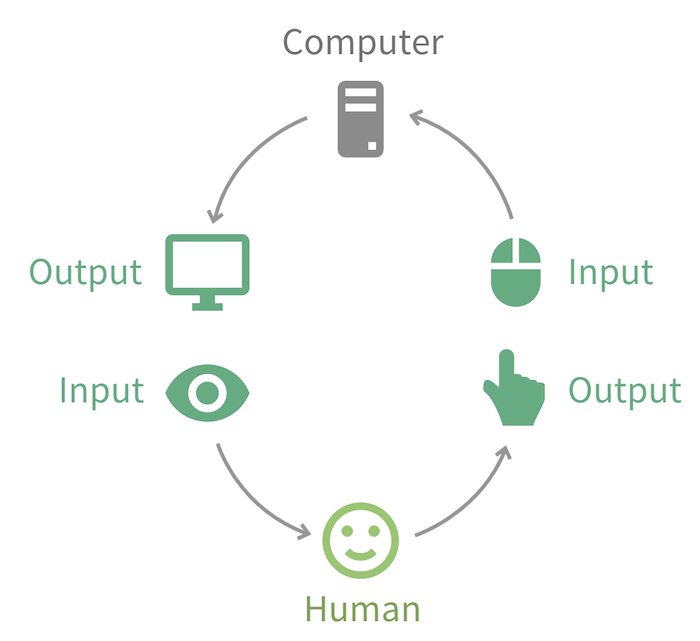
\includegraphics[height=0.5\textwidth]{./images/mvi-cycle}
    \caption{User and Computer as Input and Output}
    \caption*{Source: https://cycle.js.org/dialogue.html}
    \label{fig:userComputerInputOutput}
\end{figure}
This concept can be embodied as a chain of mathematical functions: f(g(a())) or view(model(intent(event))).
When the UI registers an event (e.g. a click) it will be passed to the intent functions as a parameter. The purpose of the intent-function is 
to translate the user generated event, as in what the user intended to do into something the application can understand and work with.
The model function then uses the output as its input. Its job is it to create a new model without changing the last one. That's what is refered to as immutability. 
\cite{immutableObjectsEffectiveJava}
It's a concept that belongs (but is not exclusive) to a programming paradigm called functional programmming
\cite{functionalProgrammingWikiHaskell,functionalProgrammingPractical,programmingInHaskellFunctionalProgrammingDefinition},
where MVI adopts ideas from.
Finally the view function receives the model as its input and takes care of rendering it (a visual representation of the model for the user). 
In order to achieve the cycle effect and the unidirectional data flow, MVI makes use of reactive programmming 
\cite{reactiveProgrammingIntroAndreStaltz} 
and the underlying "Observer" pattern 
\cite{wikipediaObserverPattern}.
\todo{why reactive, what does reactive solve for MVI? Streams?}
\todo{mention non-blocking UI?}
\todo{side effects?}
\todo{state?}
\\
To sum it up:
\begin{pquotation}{\href{https://cycle.js.org/model-view-intent.html#model-view-intent-what-mvc-is-really-about}{\nolinkurl{cycle.js.org}}, Andre Staltz}
    Model-View-Intent (MVI) is reactive, functional, and follows the core idea in MVC. It is reactive because Intent observes the User, Model observes the Intent, 
    View observes the Model, and the User observes the View. It is functional because each of these components is expressed as a referentially transparent function 
    over streams. It follows the original MVC purpose because View and Intent bridge the gap between the user and the digital model, each in one direction.
\end{pquotation}
Given the description of MVI, the questions that arises are: What does an event look like? How is immutability achieved?
Since MVI does not have a "Controller", "Presenter" or a "ViewModel": Where does the logic belong? And how is separation of concerns possible?
To summarize, it becomes a question of implementation. What does a developer have to do in order to implement or reap the benefits from this concept of MVI?

